\section{CE21B112}

\title{\textbf{Assignment 4}}
\author{\textbf{Sameer Surla CE21B112}}
\date{\textbf{June 2022}}

\maketitle
\subsection{Taylor's Series}

The Taylor series of a real or complex-valued function f(x) that is infinitely differentiable at a real or complex number a is the power series

\begin{equation}
f(a) + f'(a)\frac{(x-a)}{1!} + f''(a)\frac{(x-a)^2}{2!} + f'''(a)\frac{(x-a)^3}{3!} + ....
\end{equation} 

where n! denotes the factorial of n. In the more compact sigma notation, this can be written as

\begin{equation}
    \sum_{n=0}^{\infty} \frac{f^{(n)} (x)}{n!} (x-a)^n
\end{equation}

where $f^{(n)}(a)$ denotes the nth derivative of f evaluated at the point a. (The derivative of order zero of f is defined to be f itself and $(x−a)^0$ and $0!$ are both defined to be 1.)
\newline
\newline
When a = 0, the series is also called a Maclaurin series.
The Taylor series of any polynomial is the polynomial itself.
\newline
The Maclaurin series of 
$\frac{1}{1-x}$
 is the geometric series

\begin{equation}
    1+x+x^2+x^3+x^4+...
\end{equation}

\subsubsection{Exponential function}

The exponential function ${ e^{x}}$ (with base e) has Maclaurin series
\begin{equation}
  ln(1-x) = -\sum_{n=1}^{\infty} \frac{x^{n}}{n!} = 1+x+ \frac{x^2}{2!}+ \frac{x^3}{3!}+...
\end{equation}
It converges for all x.
\newline

\subsubsection{Natural logarithm}
The natural logarithm (with base e) has Maclaurin series
\begin{equation}
  ln(1-x) = -\sum_{n=1}^{\infty} \frac{x^{n}}{n!} = -x- \frac{x^2}{2!}- \frac{x^3}{3!}-...
\end{equation}

\begin{equation}
  ln(1+x) = \sum_{n=1}^{\infty} (-1)^{n-1}\frac{x^{n}}{n!} = \frac{x^2}{2!}+ \frac{x^3}{3!}-...
\end{equation}

They converge for $|x|<1$. ( In addition, the series for $ln(1 − x)$ converges for x=−1, and the series for $ln(1 + x)$ converges for x = 1.)\\

If f(x) is given by a convergent power series in an open disk centred at b in the complex plane (or an interval in the real line), it is said to be analytic in this region. Thus for x in this region, f is given by a convergent power series

${\displaystyle f(x)=\sum _{n=0}^{\infty }a_{n}(x-b)^{n}.}$

Differentiating by x the above formula n times, then setting x = b gives:\\

${\displaystyle {\frac {f^{(n)}(b)}{n!}}=a_{n}}$\\

and so the power series expansion agrees with the Taylor series. Thus a function is analytic in an open disk centred at b if and only if its Taylor series converges to the value of the function at each point of the disk.

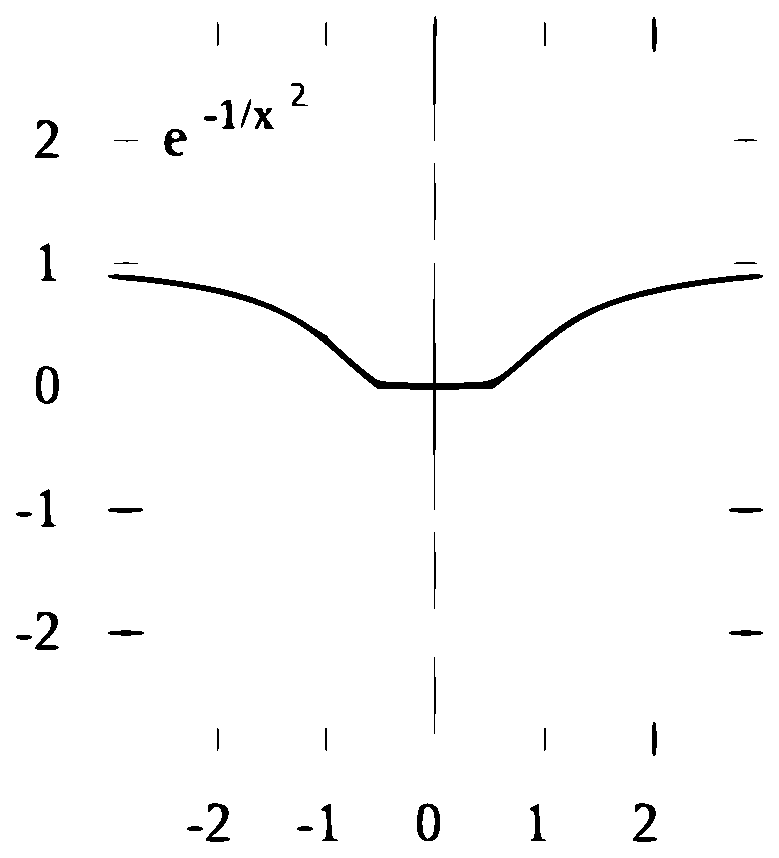
\includegraphics[scale=0.5]{450px-Exp_neg_inverse_square.svg.eps}

